\documentclass{article} 
\usepackage{todonotes}
\usepackage{graphicx}
\usepackage{algorithm}
\usepackage[noend]{algpseudocode}
\usepackage{float}
\usepackage[font=small,labelfont=bf]{caption}
\usepackage[left=0.8in, right=0.8in, top=0.9in, bottom=1in]{geometry}
\graphicspath{ {images/} }


\title{ \textbf {\vspace{0.5cm}\Huge Distributed URL-Shortener \\}
 Final Project for the Distributed Enabling Platform course \vspace{1.0cm}\\} 

\date{\vspace{2cm}}

\author{ \Large Francesco Balzano \vspace{0.3cm}\\ 
%Matricola 541533 \vspace{0.5cm}\\
\Large Master Degree in Computer Science and Networking \vspace{0.4cm} \\
\Large A.Y. 2016-2017 
}


\begin{document}
  \pagenumbering{gobble}
  \maketitle
  %\newpage
  \noindent\rule{18cm}{0.4pt}
  \tableofcontents
  \newpage
  \pagenumbering{arabic}

\clearpage
\setcounter{page}{2}
  
\section{Overview}  
URL shortening is the translation of a long Uniform Resource Locator (URL) into an abbreviated alternative that redirects to the longer URL.  A shortened URL may be desired for messaging technologies that limit the number of characters in a message, for reducing the amount of typing required if the reader is copying a URL from a print source, for making it easier for a person to remember, or for the intention of a permalink.\\  
The aim of this project is to provide the implementation of a distributed url-shortener service.


\section{Design choices}
There are three fundamental metrics in the assessment of a distributed system: Consistency, Availability and Partition Tolerance. It is well known from the CAP theorem that it is impossibile to achieve all of them at the same time in a distributed system. \\ 
In this project, I have chosen to focus on availability and partition tolerance, at the expense of consistency. In particular, the consistency model is not a strong one. Another goal of this project is to be scalable.
In the following subsections, I list and explain the design choices that I made.


\subsection{API}
The url-shortener project is a service that provides the following APIs:

\paragraph{get}
Given the shortened url returns the original url, if present. \\
\texttt{get(shortUrl) -$>$ longUrl}

\paragraph{put}
Generates and returns the shortened url associated with the provided url. \\
\texttt{put(longUrl) -$>$  shortUrl}

\paragraph{remove}
Removes the couple \texttt{<shortened url, original url>}.\\
\texttt{remove(shortUrl) -$>$  longUrl}


\subsection{Passive Replication}
Clients can communicate with every node. If the contacted node is the primary for that request, it will execute the request and directly return the result to the client; otherwise it will forward the request to the primary, which will execute it and send back the response to the sending node, which in turn will hand it back to the client. \\ 
I have chosen the Passive Replication strategy because it should keep lower the number of version conflicts with respect to active replication.

\subsection{Data Partitioning}
The partitioning strategy to map objects into nodes is a dynamic one: namely, it is employed Consistent Hashing with virtual nodes. The use of virtual nodes has potentially two advantages: in case of heterogeneous machines we can assign more virtual nodes to the most powerful machines, so that it will be more likely that these machines will handle a bigger number of items. The other advantage concerns homogeneous machines (\texttt{i.e.} machines with similar computational power, bandwidth, storage...). In this case the use of virtual nodes results in a more fair distribution of items among nodes with higher probability. \\ In case of node leave, due for instance to node crash or network partition, the keys assigned to this node are automatically assigned to another, working node. Since we have replication of data and we use the gossip protocol to detect dead nodes, we are capable to face the leave of one or more nodes without compromising the functioning of the whole system. In other words, availability and partition tolerance are guaranteed.

\subsection{Data Replication}
We want to achieve availability, so an asynchronous replication strategy is adopted. Namely, the primary node immediately answers to the client after an operation is performed. Messages to the backup nodes are sent periodically, and not after every update of the primary's data. This strategy reduces the latency of the communication client-primary, again at the expense of consistency. \\
Each primary node is associated one backup node, which is the next node clockwise in the ring. Every time a primary wishes to update its replica, it sends all the content of its database to this node. I have chosen this strategy in order to be the more scalable as possible. Each node has a primary database and a backup database. The primary database is the one used by a node to answer the requests addressed to itself. The backup database instead is used to store the replicated urls: indeed periodically the primary node sends the content of its primary database to the backup node, which stores the received urls into its backup database.

\subsection{Primary Failure}
The use of Consistent Hashing and the the specific data replication strategy adopted (backup is the next node clockwise in the ring) allows to have a very easy failover procedure: let \textit{n} be the number of nodes in the ring, if node \textit{i} is down the space of keys that belonged to node \textit{i} will be automatically mapped to node \textit{(i+1) mod n}. Since node \textit{(i+1) mod n} is the backup of node \textit{i} it will have a copy of the keys of node \textit{i} (although possibly not updated), so the correct behaviour will be maintained also in case of failure of the primary without needing an explicit failover procedure. For further details about the failover procedure please refer to the  \textit{Implementation} section.    


\subsection{Consistency Model}
This project adopts an eventual consistency model. It is possible to get different results if running the same query at the same time on the leader and on a follower. This may happen if the follower has an outdated version of the leader's data. Anyway this is only a temporary state: if we stop writing to the database for a while, the followers will eventually become consistent with the leader. I decided to accept this weak consistency model in order to have better availability and partition tolerance. Furthermore, in absence of failures only the leader answers to requests for which it is the primary, and so inconsistencies do not arise.

\subsection{Conflicts Resolution}
Each node is assigned a vector clock that allows it to order events, that is to track causal dependencies between events. When a message is sent from a node to another, it carries both the object (the target of the communication) and the sender's vector clock. If the recipient node already has that object with the associated vector clock in its database, two situations may arise:
\begin{itemize}
\item  If one vector clock is smaller than the other, keep the greatest (i.e. latest) version of the object;
\item  If that is not the case, the two vector clocks are concurrent, and if the two objects are assigned different values then we have a conflict.
\end{itemize}
In case of conflict I have adopted a \textit{last write wins} approach: each object carries also a timestamp, so if the vector clocks are concurrent the object with more recent timestamp is kept. This method is prone to data loss but I decided to adopt it because of its simplicity and because with a Passive Replication Strategy conflicts should be rare. In particular, in this system it is possible to have conflicts only when a node recovers from failure and its backup node has processed requests such that now the state of the backup and of the primary node is inconsistent. I discuss this problem and the adopted solution in the \textit{Conflict Resolution} paragraph of the \textit{Test} section, where I also provide tests to check the correctness of the approach.



\section{Implementation}  
There are clients, that invoke the service, and nodes, that comprise the cluster and actually implements the service. Clients and nodes stay in two different modules: the formers in the client module, the latters in the core module. Indeed they are logically different things, and so they should be able to evolve independently from each other. 

\subsection{Architecture} 

The client can make a request to any node in the cluster. The nodes process the request and handle back the result to the client. In particular, only the primary node for a given request actually processes it. If a node receives a request for which it is not the primary, it discovers who is the primary and forwards the request to such node. The primary node processes the request and then handles back the result to the previous node, who in turn returns the response to the client. \\
Each node has to do three main jobs, so I created a node as a container of three services: 
\begin{itemize}
\item \textit{client communication service}: each node must be able to communicate with the client, to accept requests from it and return responses;
\item \textit{node communication service}: each node must be able to communicate with the other nodes. Indeed, it could have to forward the client request to the primary node, or to send the content of its own database to the backup node, or even only to check that the other nodes of the cluster are alive;
\item \textit{storage service}: each node must have a database, to store and retrieve urls on client's behalf. Actually, it has two databases: its own database, used to handle requests, and the backup database, used to replicate the data of another node. The reason for the use of two distinct databases is explained in \textit{``The core module''} paragraph. 
\end{itemize}
Figure \ref{fig:architecture} shows the architecture of the service. The communication between client and nodes exploits TCP, both because I assume an unreliable communication channel between them and because of \textit{interactive} sessions. Indeed the possibility of starting an interactive service session between the client and a node amortizes TCP overhead, since the same amount of overhead will be payed (to open and close the connection) no matter how many times the service is invoked by the client. Instead, communication among nodes in the cluster uses UDP for the opposite reasons. First, I assume a much more reliable network inside the cluster. Second, usually single messages are sent from a node to another, and so establishing a TCP connection to send only one message would be too costly.

\begin{figure}[h]
\centerline{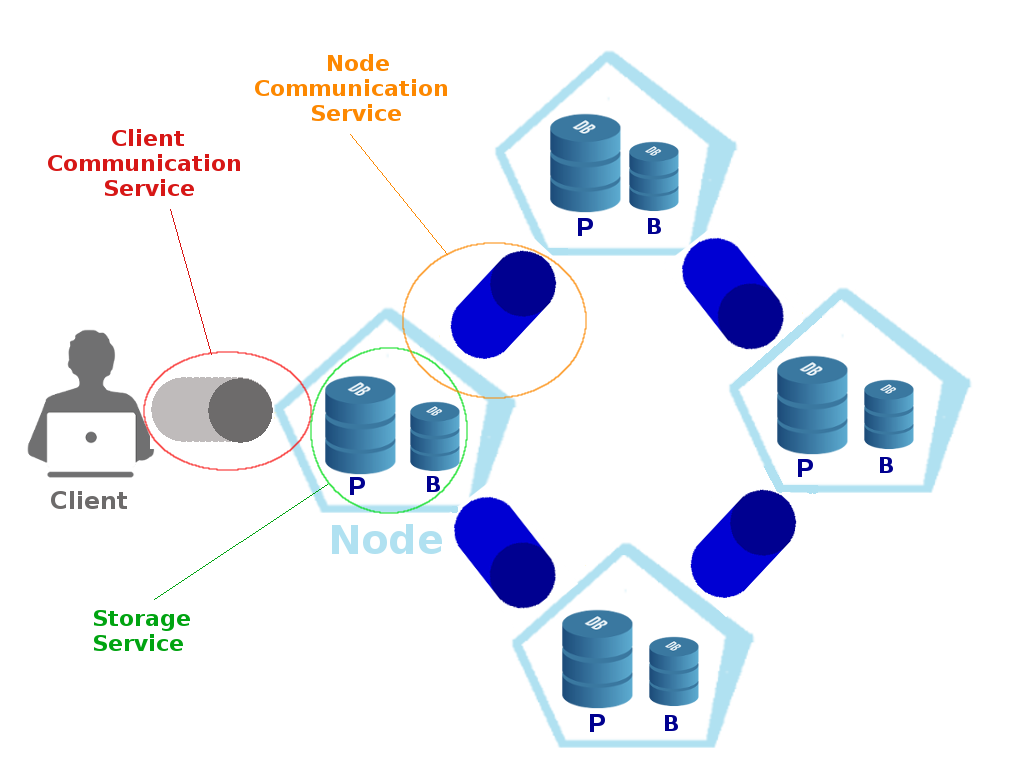
\includegraphics[scale=0.41]{architecture}}
\caption{General architecture. There is a client and a cluster, which is made of four nodes. Each node is made of a node communication service, a client communication service and a storage service. The letter ``P'' under the database stays for ``primary'' , the letter ``B'' for ``backup''.}
\label{fig:architecture}
\end{figure}

\subsection{The project classes} 
The structure of the project is the following. The node is the building block of the cluster and, as we already said, it is made of three main \textit{services}. Each of these services provides a high level view of the functionalities it has to implement. For the actual implementation these services rely on proper \textit{managers}, which have the responsability to setup things and handle lower level details. Figure \ref{fig:class_diag} shows a simplified UML class diagram, in which the relationships among classes are highlighted (but not the methods). In particular, this diagram only shows the classes of the \textit{core} module, because it is this module that implements the logic of the service. Instead the \textit{client} module only parses the user's request and sends it to proper classes of the core module to be processed. \\




\subsubsection{The core module} 
The core module contains all the classes that implement the logic of the project. The Node class is the main class and the building block of the cluster. This module contains classes and methods to receive and process client requests, find the primary node for any request, handle the partition and replication of data, cope with node failure and resolve conflicts. Classes inside this module are organized into the following packages: \textit{communication, message, storage} and \textit{utils}. Some classes belong to the \textit{core} package but not to any of the mentioned subpackages. I start describing these classes, and then I pass to the classes in the subpackages. \\
\begin{itemize}
\item \textit{NodeRunner} It is the class that actually runs the url-shortener service. Indeed it setups the cluster by setting the configurations specified in the configuration file.
\item \textit{CoreCommandLineManager} Parses the command-line input and provides methods to deal with the options that can be specified from command-line.
\item \textit{Node} A node is made of a \textit{ClientCommunicationService}, a \textit{NodeCommunicationService} and a \textit{StorageService}. A cluster is simply a collection of interacting nodes. 
\item \textit{Service} A simple \textit{Interface} for the various services, that only states that each service must provide a \textit{start()} and a \textit{shutdown()} method.
\end{itemize}

\paragraph{communication} The Communication package gathers classes that are involved in the communication either with clients or with other nodes. For this reason, the classes inside this package are organized in two further subpackages \textit{client} and \textit{node}. 
\subparagraph{client} 
\begin{itemize}
\item \textit{ClientCommunicationService} One of the three fundamental services a node is made of. It starts and shuts down a ClientCommunicationManager.
\item \textit{ClientCommunicationManager} It listens on a TCP ServerSocket to accept client requests. As soon as a request is received, a ClientCommunicationThread is created and run to handle it. Then, the ClientCommunicationManager continues to listen on the socket for further requests. It also provides a method to process the client request, by delegating the processing to the NodeCommunicationManager.
\item \textit{ClientCommunicationThread} It communicates with the client by using the socket received from ClientCommunicationManager. In particular, it receives the client message, asks the ClientCommunicationManager to process it and finally returns the result to the client.
\end{itemize}
\begin{figure}
\centering
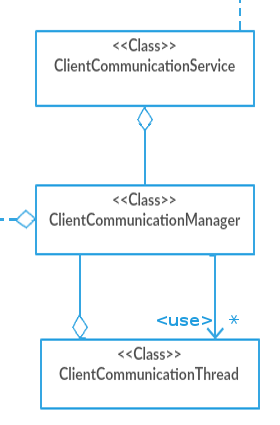
\includegraphics[scale=0.40]{classes_client_subpackage}
\caption{UML class diagram, showing up relationships among classes in the core.communication.client subpackage}
\label{fig:class_diag_core.communication.client	}
\end{figure}

\subparagraph{node} 
\begin{itemize}
\item \textit{NodeCommunicationService} One of the three fundamental services a node is made of. It starts and shuts down a NodeCommunicationManager.
\item \textit{NodeCommunicationManager} It is the responsible for the communication among nodes. It starts and shuts down the RequestManager and the ReplicaManager, and provides the capability to process the client messages it receives. In particular, if it is the primary for that request it will ask the StorageService of the node to perform the proper operations; otherwise it will discover the primary node and forward the message to it.
\item \textit{RequestManager} NodeCommunicationManager relies on this class to actually receive and send requests among nodes. A Request is intended as any message that can be received or sent by a node. It can be a client message, a node message or an update message. The RequestManager acts both as server and client for the request: to manage incoming requests it spawns a RequestServerThread while to make outgoing requests it provides a \textit{sendMessage()} method that spawns a RequestClientThread to do the job. It continously listen on a UDP socket.
\item \textit{RequestServerThread} It reconstructs the message from a stream of bytes, delegates the MessageHandler to properly process the message, collects the reply and sends it back to the requesting node via UDP.
\item \textit{RequestClientThread} This class is symmetric with respect to RequestServerThread, in the sense that it is the class that starts the message exchange with another node in the cluster.
\item \textit{ReplicaManager} Periodically sends the content of the database to the backup node. If we look at nodes in the cluster as points in a ring, the node to whom send the database is the next node clockwise in the ring. To update the backup database the ReplicaManager splits its own database in fixed-size pieces: each of these pieces will be encapsulated in an UpdateMessage and sent to the backup node. To send these update messages the ReplicaManager relies on the RequestManager, because an UpdateMessage is simply seen as a request.
\end{itemize}
\begin{figure}
\centering
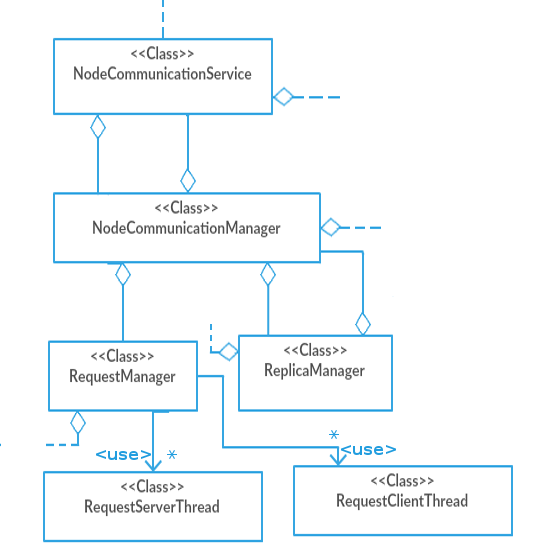
\includegraphics[scale=0.40]{core_communication_node}
\caption{UML class diagram, showing up relationships among classes in the core.communication.node subpackage}
\label{fig:class_diag_core.communication.node	}
\end{figure}

\paragraph{message} A Message is the base interface for communications. Following the layout of the project, three further interfaces are defined, that inherits from Message: ClientMessage, NodeMessage and UpdateMessage, to deal respectively with client messages, node messages and database backup. 
\begin{itemize}
\item \textit{Message} Base interface: implementing classes must provide methods to return the status (success, error, ...) and the type (put, get, ...) of the message.
\item \textit{ClientMessage} Interface for client message: implementing classes must provide a method to get the url inserted by the client.
\item \textit{GetMessage} Class that implements ClientMessage, it is used when GET requests are invoked by the client.
\item \textit{PutMessage} Class that implements ClientMessage, it is used when PUT requests are invoked by the client.
\item \textit{RemoveMessage} Class that implements ClientMessage, it is used when REMOVE requests are invoked by the client.
\item \textit{NodeMessage} Interface for the messages generated by the nodes from the client messages. Implementing classes must provide methods to retrieve the original url, the associated shortened url and the vector clock associated to those urls.
\item \textit{VersionedMessage} Class that implements the NodeMessage interface.
\item \textit{UpdateMessage} Interface used when portions of the database are sent to the backup node. Implementing classes must provide methods to put and get entries of the database in the message, check whether the UpdateMessage is full or empty, return the identifier of the sender node and tell whether this message is the first of a sequence of UpdateMessage. Indeed, the content of a backup is delivered by sending a sequence of UpdateMessages, and the first message may need some special treatment.
\item \textit{SizedBackupMessage} Class that implements the UpdateMessage interface. Its name means that it is involved in backup operations and that can carry only a limited amount of database entries (indeed these messages have to be sent over UDP).
\end{itemize}
\begin{figure}
\centering
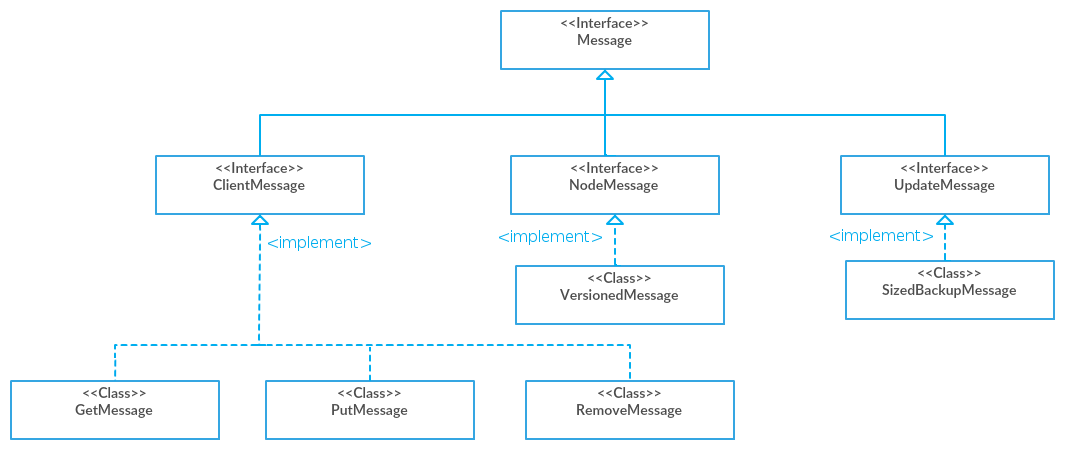
\includegraphics[scale=0.4]{core_message}
\caption{UML class diagram, showing up relationships among classes in the core.message subpackage}
\label{fig:class_diag_core.message}
\end{figure}

\paragraph{storage} The classes inside this package deals with database operations.
\begin{itemize}
\item \textit{StorageService} It starts and shuts down the StorageManager. It is not directly involved in any operation concerning the database.
\item \textit{StorageManager} It is the class that actually manages the database. The database is a simple \textit{(key,value)} store, whose keys are \textit{short urls} and whose values are \textit{versioned long urls}, that is the original url paired with a vector clock and a timestamp. Each node has two databases: a primary and a backup database. The primary database is the one that contains the urls for which the node is the primary. So every time the StorageManager is asked to answer to a client request, it looks in the primary database. The backup database instead contains a copy of the primary database of another node. Namely, according to the chosen replication strategy, the backup database of node \textit{i} contains the copy of the primary database of node \textit{(i-1) mod N}, where N is the cluster size. The backup database is never used to answer clients' query. The backup database of node \textit{i} is periodically updated by node \textit{(i-1)} through the sending of a sequence of UpdateMessages. Upon receiving these messages, the recipient node checks whether the sending node is the same of the last time (this is possible because the UpdateMessage has a field that stores the id of the sending node). If it the same, the backup database is updated and everything is fine; if it is different, it means that either node \textit{(i-1)} crashed or recovered from crashing (I assume that new nodes cannot join the cluster, but obviously crashed or partitioned nodes can re-join it). In case of crashing or partitioning of node \textit{(i-1)} the node \textit{i} merges the backup database into the primary database, because now it must behave as primary also for the urls of the crashed node. So the system is partition tolerant, because it keeps working despite the failure of a node in the cluster. When node \textit{(i-1)} re-joins the cluster, the situation previous to the failure is re-established, with node \textit{i} storing again the backup database of node \textit{(i-1) mod N}. A StorageManager provides methods to read and write single entries of the database, make a dump of the primary database and merge the backup database into the primary. 
\end{itemize}

\paragraph{utils} This package contains classes that provide methods that don't fall in one of the previous categories, but may be needed by different classes. 
\begin{itemize}
\item \textit{Utils} Provides static methods to serialize and deserialize an Object and to shorten the original url. The url-shortener method exploits the 32 bit MurmurHash3 function.
\item \textit{MessageHandler} Provides static methods to process the messages. Those methods always require the StorageService to be passed as parameter, because some operation will be done on the database. Which operation depends on the type of message: PUT, GET, REMOVE and UPDATE messages get a different treatment. If MessageHandler receives a PUT message, it stores a pair \textit{(key,value)} in the primary database; if it receives a GET message a pair is read from the primary database; if it receives a REMOVE message a pair is removed from the primary database; if it receives an UPDATE message the backup database is updated with the entries contained in the message.
\item \textit{Partitioner} The Partitioner uses the ConsistentHasher class to map the urls into a space which is partitioned among nodes, such that each node will manage the urls that follow in its partition. This is what is called ConsistentHashing. The ConsistentHasher class allows us to define a given number of virtual instances per node. This means that if we decide to give 50 virtual instances to a node, that node will be assigned 50 different (and smaller) partitions.
\end{itemize}



\subsubsection{The client module} 
This module contains the classes that implement the client. The client chooses a node of the cluster and invokes an operation among PUT, GET and REMOVE. The client can establish a connection with a node that only lasts the time needed to carry out the requested operation, or an interactive session can be started, during which the connection is kept alive and the client can make as many requests as it wishes. The classes belonging to this module are the following:
\begin{itemize}
\item \textit{Client} A simple interface for the client, stating that implementing classes must provide the method \textit{sendRequest} \textit{(Message msg)} to send the request to a node of the cluster. The policy used to select the node is implementation-dependent.
\item \textit{RandomClient} A class that implements the Client Interface. Every time RandomClient has to send a message to a node, the recipient node is randomly selected among the nodes of the cluster. It uses a ClientConfig to get the list of nodes comprising the cluster.
\item \textit{ClientConfig} This class holds configuration parameters for the client. In particular, it parses the configuration file to retrieve the addresses of the nodes comprising the cluster. Such addresses are stored in a list, which is returned to the client upon request.
\item \textit{CommandLineManager} It parses the command line arguments, checking that nothing is missing and that the provided options are legal. Provides methods that ClientRunner uses to check the presence of such options and to display help or error messages.
\item \textit{ClientRunner} Runs the client, either in batch or interactive mode, and returns the result. 
\end{itemize}


\begin{figure}
\centering
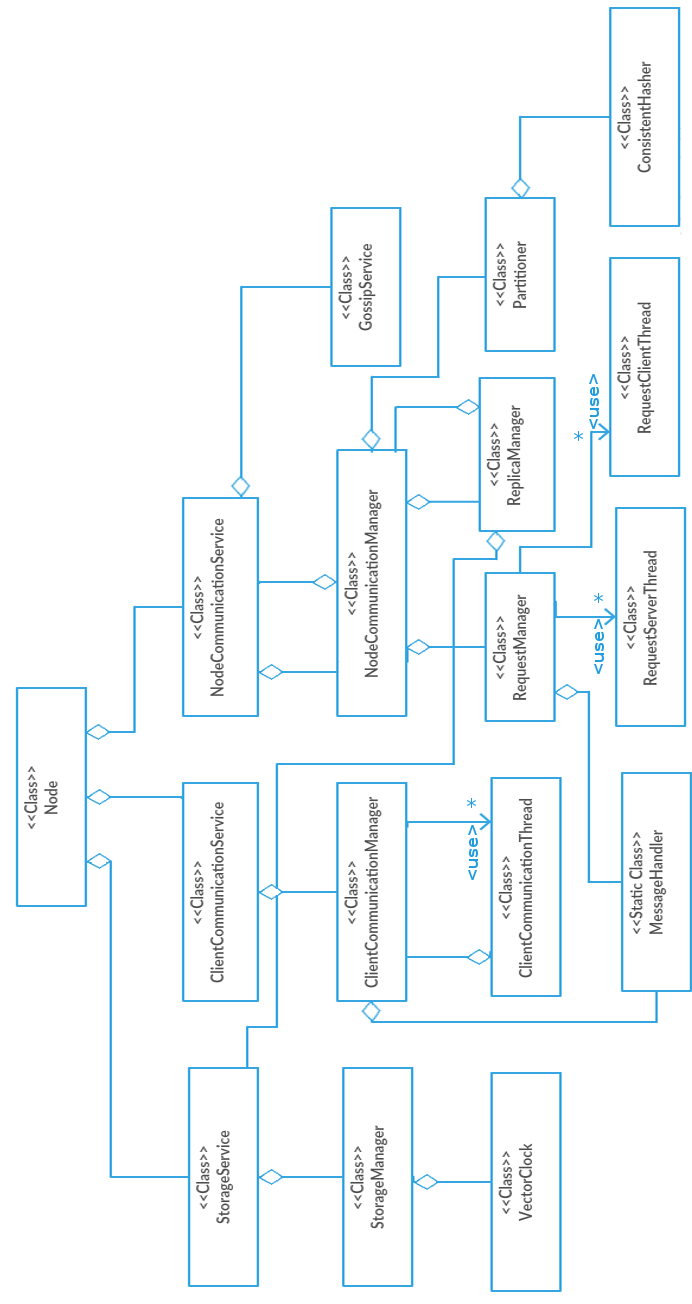
\includegraphics[scale=0.43]{core_diagram}
\caption{Uml Class Diagram of the core module. It is shown the internal composition of the node, which is the building block of the cluster. A node is made of a NodeCommunicationService, a ClientCommunicationService and a StorageService. In turn, these services rely on proper managers, who actually implement the functionalities of the services. Where omitted, cardinalities are 1.}
\label{fig:class_diag}
\end{figure}

\subsection{Use cases} 
In this section I show how the objects of the project cooperate in some common use case. Actually there is one general use case, that is the invocation of an API by the client. Indeed, despite all the possible configurations (interactive or batch, use default or custom configuration file, ...), invoking an operation among PUT, GET and REMOVE is the only thing a user can do. All the other things that the system does, like keeping updated the backup database, being partition-tolerant, resolve conflicts and so on, are transparent to the user and so do not fall in the use cases. Instead, they will fall in the \textit{Test} section.

\subsubsection{Processing of a PUT request} 
We analyze how the objects interact in case of a PUT request from a Client. The choice of PUT is arbitrary, since the pattern of message exchanges and method invocations is almost the same also with GET or REMOVE requests. The only thing that changes is obviously the operation on the database.
Let's refer to figure \ref{fig:sequence_diagram_complete}. Although we are dealing with use cases, I will not use a use case diagram because it is too high level. Instead, I want to show how the objects interact to process a client request, and so I will take advantage of a sequence diagram. We can see that three actors are involved in the request processing: the client, a first node and a second node. Indeed, we consider the most general case in which the client contacts a node which is not the primary for the given url.
So let's start reading the diagram. The ClientRunner parses the command-line to get the request together with the original url, wraps them in a ClientMessage and invokes the \textit{sendRquest(cmsg)} method on the Client, which result in opening a socket to send the message to the ClientCommunicationManager of Node 1. The ClientCommunicationManager, which is waiting for connections on a Socket, instantiates and run a ClientCommunicationThread to handle the request, passing it a reference to itself. This reference is exploited for the callback of the method \textit{processMessage(cmsg)}, which in turn results in the invocation of method \textit{processClientMessage(cmsg)} of NodeCommunicationManager. NodeCommunicationManager creates the short url from the original url carried in the ClientMessage, then uses this short url to discover who is the primary node. At this point it discovers that it is not the primary node: so it creates a NodeMessage carrying the original url, the short url and a vector clock. Finally it instantiates a RequestClientThread to send this NodeMessage to the primary node. This message is received by the RequestManager of Node 2 (that is the primary node), which is always listening for NodeMessages (or UpdateMessages) on a socket. The RequestManager instantiates and run a RequestServerThread to process the NodeMessage, which invokes the method \textit{handleMessage(nmsg)} on MessageHandler. This method discovers that it is dealing with a PUT request, and so it invokes the private method \textit{processPutMessage(nmsg)}, which exploits the StorageService to store the pair \textit{(short url, original url)} in the primary database. If the store is successful, a message with type=REPLY and status=SUCCESSFUL will be returned to the client, following back the chain of invocations. \\ The figure \ref{fig:sequence_diagram_complete} is a bit simplified, for instance the signatures of the methods are not complete, the StorageService does not directly provides a \textit{store} method (which is offered by StoreManager), and new threads are not directly created (instead it is used an ExecutorService to improve performances). I thought that these further details would have made more complex the diagram without carrying more benefits, so I have preferred a simpler but clearer diagram.	



\begin{figure}
\centering
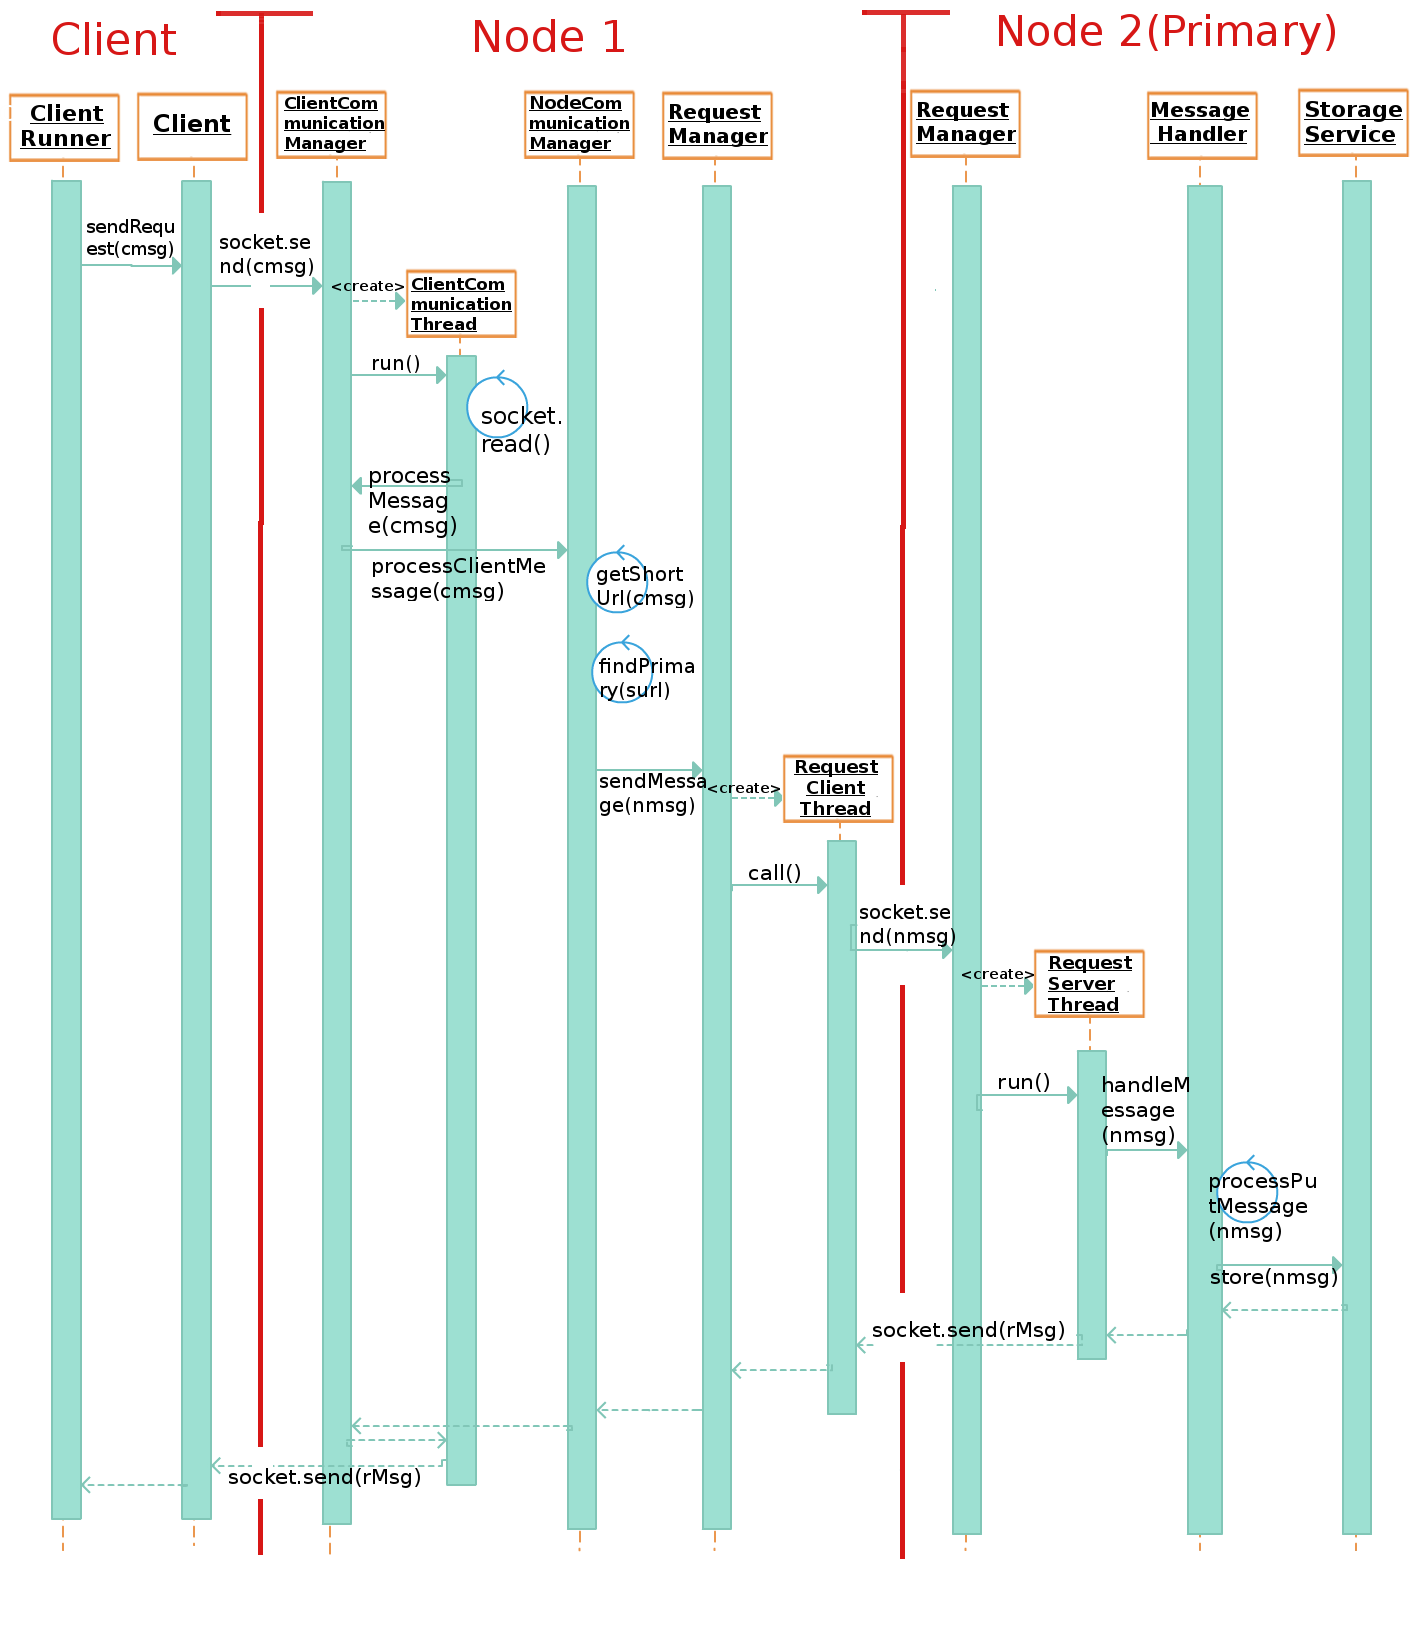
\includegraphics[scale=0.32]{sequence_diagram_complete}
\caption{Sequence diagram for the processing of a PUT request, when the node contacted by the client is not the primary.}
\label{fig:sequence_diagram_complete}
\end{figure}


\section{Test}
The tests that I provide are more similar to functional tests rather than unit tests. The reason is that I didn't want to provide a lot of trivial tests, but instead I preferred to put more complex tests, such that if they succeed, it is likely that the system works as expected. One point concerning all tests is that they generally deal with faulty situations and their successful completion depends on time. Indeed, new information does not spread immediately among the nodes. Indeed in case of node crash we have to wait that the gossip service of the nodes recognize that one node is down, to properly adapt the behaviour of the system. Furthermore we saw that information is not replicated immediately upon generation, but periodically. In addition, the use of UDP may imply that the delivery of the database to the backup node from the primary node is unsucessful. In this case, the exchange is lost and the next exchange will not be performed soon after, but when the time period elapses. The result is that the system keeps working despite failures, but it may be the case that you have to wait a while to get consistent answers. I would also highlight that this behaviour only happens in case of failure: if no one of the node fails (both for a network partition or a node crash), the system promptly provides consistent results to user queries. \\
I used JUnit 4 as framework for the tests. The classes used for the tests are \textit{DataReplicationTest}, \textit{PrimaryFailureTest} and \textit{ConflictResolutionTestTest}. Before the execution of the test, a cluster made of 5 nodes is built and after the execution of each test it is torn down, in order to have a clean environment for each test.


\subsubsection{Replication of data}
The test class is \textit{DataReplicationTest}. This test checks whether data replication actually takes place. A url is inserted in the system, by simulating a PUT request of a client. The system will find the primary for that request and will store it into the primary database of the primary node. This test checks whether, after waiting a while, this url is replicated into the backup database of the backup node.

\subsubsection{Primary failure} 
The test class is \textit{PrimaryFailureTest}, the test function \textit{backupShouldReplacePrimary()}. In this test we show that the system reacts correctly in case of primary failure, without needing any manual intervention. The situation is analogous to the case of network partition of the primary. 
A url is inserted in the system and is stored in the database of the designated primary node. Then we wait for the primary to replicate its database into the backup node and we shut down the primary to simulate a failure. At some point the backup node will receive an UpdateMessage from a node different from its primary. The backup node understands that the primary is down and that it must start to manage the requests of the failed primary too, so it merges its backup database into its primary database, that is it copies the urls in the backup database into the primary database. The test checks that if we make a request for the url inserted before, and the primary is down, the request is successfully answered by the backup node.




\subsubsection{Primary re-joins cluster after failure} 
The test class is \textit{PrimaryFailureTest}, the test function \textit{primaryShouldWorkWhenRejoiningCluster()}. In this test we show that the system works correctly when the primary node re-joins the cluster after crashing, that is it is assigned the same space of urls that it had before crashing. The situation is analoguos to the case of primary re-joining the network after a partition.
This test takes the previous one a step further, that is: a url is inserted in the system, some time is waited to allow the replication of data from primary to backup node, the primary node is shut down, some time is waited (during which the backup node manages the requests of the failed primary too), and finally the primary node is restarted. This test checks whether after rejoining the cluster, the primary node is able to return the url previously inserted in the system.

\subsubsection{Conflict Resolution} We need to spend more words on conflict resolution to show when conflicts may arise, how they are managed, and which are the tests employed to check whether the system handles conflicts as expected.
\paragraph{Birth of a conflict} The system exploits a Passive Replication strategy. This means that only the primary node processes the requests it is responsible for. Backup nodes only forward the requests to the primary node: they do not directly process the requests for which they are not primary. This approach implies that in absence of failures, no conflict can arise. So, conflicts can happen only when a node recovers from crashing if during the time in which it was down its backup node has processed some requests that lead to an inconsistent state between the database of the primary and the database of the backup. Namely this can happen if the backup node has removed or updated some urls while the primary node was down. Figures \ref{fig:conflict1}, \ref{fig:conflict2} and \ref{fig:conflict3} show the sequence of actions that may lead conflicts. 

\begin{figure}
\minipage{0.45\textwidth}
  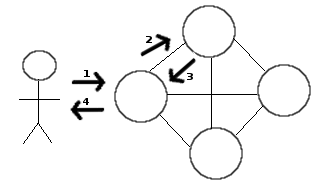
\includegraphics[width=\linewidth]{conflict1}
  \caption{Behaviour of the system in absence of failures: the request is processed by the primary.}\label{fig:conflict1}
\endminipage\hfill
\minipage{0.45\textwidth}
  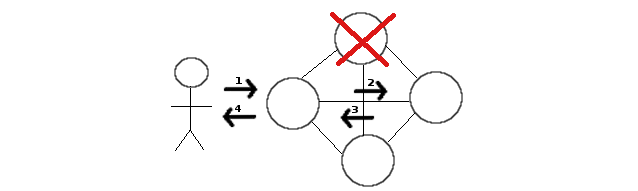
\includegraphics[width=\linewidth]{conflict2}
  \caption{Behaviour of the system in case of failure of the primary: the requests are processed by its backup node.}\label{fig:conflict2}
\endminipage\hfill
\end{figure}

\begin{figure}
\centering
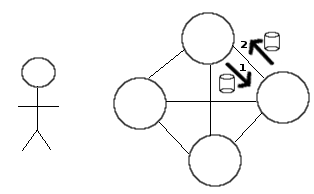
\includegraphics[scale=0.45]{conflict3}
\caption{The failed node is recovered and re-joins the cluster. The backup node discovers that the primary is alive again as soon as it receives an UpdateMessage from it. At this point the database received from the primary is discarded by the backup node, because it contains outdated information. Instead, the backup node sends to the primary the collection of urls that from now on will be managed by the primary.}
\label{fig:conflict3}
\end{figure}

\paragraph{Conflict management} Let's assume that now we are at the point in which the backup node is processing the requests addressed to the  primary, when the primary node suddenly recovers from failure and re-joins the cluster. The backup had discovered that the primary was down when it received the database to be replicated from a node different from its default primary. At that point it merged its backup database into the primary database, in order to be able to process also the requests of the failed node. Now it discovers that its default primary node is again alive, but probably there are inconsistencies among the primary databases of the two nodes. With reference to figure \ref{fig:sets}, it is possible to distinguish three cases:
\begin{itemize}
\item \textit{(1)} Urls in the database of the primary node BUT NOT in the database of the backup node. If this situation arises because these urls were not sent to the backup node because the primary node had failed, then the primary node must keep those urls. Instead, if this urls are not present in the database of the backup node because they were removed while the primary node was down, then they have to be removed from the database of the primary too.
\item \textit{(2)} Urls in the database of the primary node AND in the database of the backup node. It could be the case that both backup node and primary node have the same keys (short urls), but the values (long urls) are different because those url have been updated by the backup node while the primary node was down. So, all the urls belonging to this subset have to be sent to the primary node, which will run a conflict resolution procedure to solve possible conflicts among urls having the same key but different value.
\item \textit{(3)} Urls in the database of the backup node BUT NOT in the database of the primary node. The backup node sends to the primary node only those urls that now have to be managed by the primary.
\end{itemize}
These cases are handled by algorithms run both by the backup node and by the primary node. The backup node runs the algorithm as soon as it receives a message from its default primary node, that it believed crashed. The primary node instead runs the algorithm as soon as it receives the message sent from its backup node. The pseudocode capturing the main ideas of the algorithms is reported below. One point has to be explained of algorithm \ref{pa}. A url sent by the backup node to the primary node has value (i.e. long url) \textit{null} if and only if that url has been removed from the backup node. In other words a url with value equal to null is a url that belonged to the data structure \textit{removedUrls} in algorithm \ref{ba} and so it has to be removed from the database of the primary node too. The method \textit{storeWithConflictResolution} uses vector clock to resolve conflicts among the stored urls and the received urls. If a \textit{happen-before} relationship does not hold between the two conflicting urls, then vector clocks cannot be used to resolve the conflict. In this case a last write wins approach is adopted, and the url with more recent timestamp is kept.

\begin{algorithm}
\caption{Algorithm run by backup node}\label{ba}
\begin{algorithmic}[1]
\If  {(defaultPrimary == updateMsg.sender AND actualPrimary != defaultPrimary)}  
\State backupDB.empty()
\State partitionUrlsBetweenDB()
\State backupDB.add(removedUrls)
\State actualPrimary = defaultPrimary
\State send backupDB to node defaultPrimary
\EndIf 
\end{algorithmic}
\end{algorithm}


\begin{algorithm}
\caption{partitionUrlsBetweenDB()}\label{purls}
\begin{algorithmic}[1]
\For {$<$surl, lurl$>$ in primaryDB} 
\If {(findPrimary( surl ) != me)}
\State primaryDB.remove( $<$surl, lurl$>$ )
\State backupDB.store( $<$surl, lurl$>$ )
\EndIf 
\EndFor
\end{algorithmic}
\end{algorithm}

\begin{algorithm}
\caption{Algorithm run by primary node}\label{pa}
\begin{algorithmic}[1]
\For {$<$surl, lurl$>$ received from backupNode}
\If {($<$surl, lurl$>$ $\notin$ primaryDB )} \Comment{Case 3}
\State primaryDB.store( $<$surl, lurl$>$ )
\Else 
\If {(lurl == null)} \Comment{Case 1}
\State primaryDB.remove( $<$surl, lurl$>$ )
\Else { storewithConflictResolution( $<$surl, lurl$>$ )} \Comment{Case 2}
\EndIf
\EndIf 
\EndFor
\end{algorithmic}
\end{algorithm}


\begin{figure}
\centering
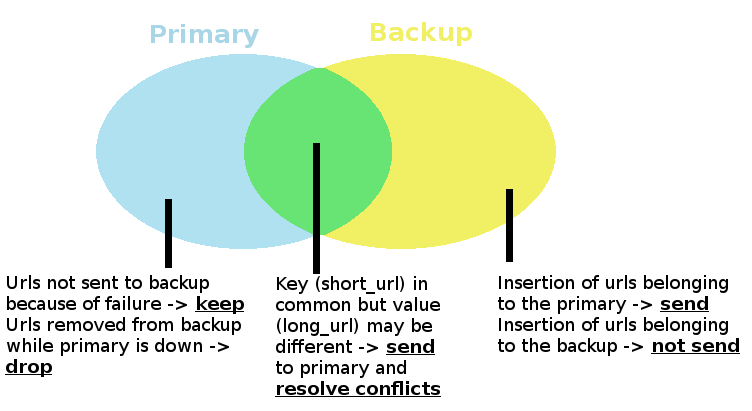
\includegraphics[scale=0.45]{sets}
\caption{Cases that have to be managed when the primary node recovers from crashing}
\label{fig:sets}
\end{figure}


\paragraph{Tests} The test class is \textit{CoflictResolutionTest}. Inside this class, two tests are present:
\begin{itemize}
\item \textit{primaryShouldResolveConflictsAfterRejoiningCluster()} This test checks whether the primary node resolves conflicts as expected. A url is inserted in the database of the primary node and some time is waited to allow the replication of the database in the backup node. Then the primary node is shut down and some time is waited to allow the backup node to understand that it must handle also the urls of the failed node. At this point the value of the previous url is modified by the backup node and then the primary node is restarted. At some point the primary node will contact again the backup node, which understands that its default primary is up again. The backup node sends to the primary node the updated url. The primary node recognizes that it has already stored that url in its database and runs the conflict resolution procedure. If the system works as expected, the primary node replaces the old value of the url with the new value received from the backup node (when I talk about value of the url I mean the long url: indeed the urls are stored in the database as pairs \texttt{$<$surl, lurl$>$}, so the short url can be seen as key and the long url can be seen as value of the pair).
\item \textit{primaryShouldRemoveUrlsRemovedByTheBackupNode()} This test checks whether the primary node removes the urls that were removed from the backup node while it was down.
\end{itemize}

\section{Limitations} 
\begin{itemize}
\item Hash function for the url shortener. \\
The 32 bit hash function used allows about 4 billions of distinct urls. If a lot of urls have to be shortened, it must be used a hash function that maps the long urls in a bigger space. As an example, it could be exploited the 128 bit Murmurhash3 function.
\item Replication Strategy. \\
Every time the backup database has to be updated, the whole database is emptied and then rebuild from scratch. This is a simple approach (the sending node sends all its database and not only the entries that have changed from the last database delivery) but not very efficient.
\item Eventual Consistency. \\
Sometimes the system is slow at reaching consistency. If you run the tests decreasing the waiting time, it is likely that the tests will not succeed.
\item Replica management. \\
I designated the project with scalability in mind, that's why I avoided a replication strategy based on multicast. Anyway the solution I devised obliged me to put ad-hoc code to deal with special situations (\textit{e.g.} when a node remains alone in the cluster, when one node fails, ... ) making the code longer and more bug-prone.  
\item Partition Tolerance. \\
Since in the cluster all nodes are connected with all the others, I considered that only disconnections of single nodes may happen. The system supports more than one simoultaneous (single) disconnections, but I didn't test what happens in case of a disconnected components with more than one node.
\end{itemize}

\end{document}
